\section{L'analyse des liens}
\begin{itemize}
\item Concentrateurs (\textit{Hubs})
\item Autorités (\textit{Authorities})
\item Comment trouver la meilleure page ? (Voir figure \ref{fig-14-1}	)
\end{itemize}



\begin{figure}[!h]
\centering
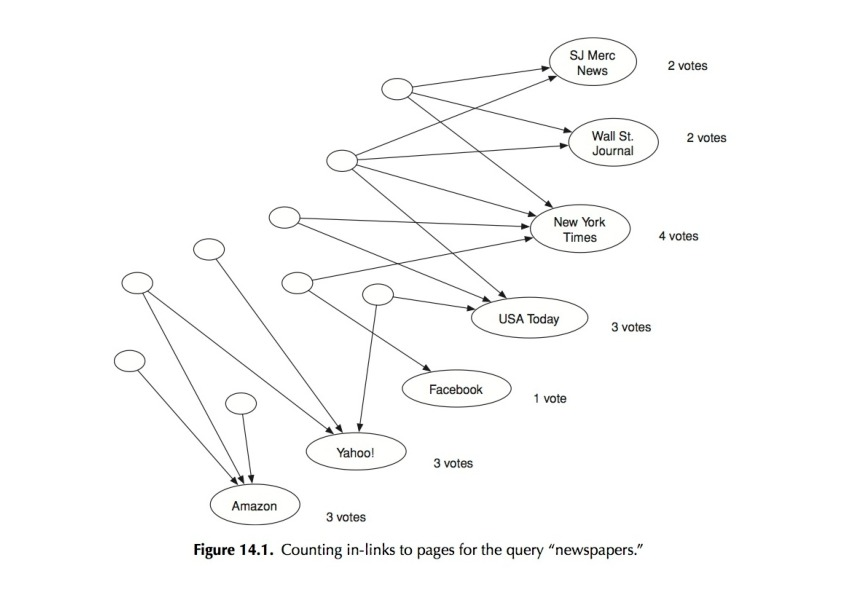
\includegraphics[scale=0.5]{images/ref/fig-14-1.jpeg}
\caption{Comptage des liens entrants pour la recherche "newspapers"}
\label{fig-14-1}
\end{figure}

\subsection*{Requête "newspapers"}

\paragraph{Pourquoi Facebook, Yahoo, Amazon, se retrouvent-ils dans la requette News Papers ?}
Car beaucoup d'utilisateurs ont des pages concentrées sur ces sites et comme dans cet exemple on utilise un algorithme qui n'est pas très sophistiqué, elles apparaissent. 

\paragraph{Comment trouver la meilleure page ?}
\begin{enumerate}
\item Compter les liens entrants comme une estimateur de la qualité d'une autorité.
\item Classer les concentrateurs en fonction de la qualité des pages qu'elles référencent.
\item Mettre à jour la qualité des autorités en fonction du poids de la source des liens.
\item Mettre à jour les concentrateurs.
\end{enumerate}

\subsubsection{Algorithme}

\begin{itemize}
\item Pages autorité (liens entrants) $ \rightarrow $ auto (p)
\item Pages concentrateurs (liens sortants) $ \rightarrow $ conc (p)
\item Mises à jour des liens entrants:
\begin{align*}
 auto'(p) =   \sum_ {p'\rightarrow p}conc(p') &&
\text{\emph{avec $p'\rightarrow p $ les pages p' qui ont un lien vers P}}
\end{align*}

\item Mises à jour des liens sortants: 
\begin{align*}
conc'(p) = \sum_ {p\rightarrow p'}auto(p') &&
\text{\emph{avec $p \rightarrow p' $ les pages p' qui sont référencées par p}} 
\end{align*}

\end{itemize}



\subsubsection*{Itération}}

$$
\forall~p~in~pages :
\left \{
\begin{array}{l}
auto(p) = 1 \\
conc (p) = 1 

\end{array}
\right.
$$

 Mise à jour, normalisation :
 
 \begin{align*}
 auto'(p) = \frac{auto (p)}{\sum auto(p')}
 \end{align*}
 \begin{align*}
 conc' (p) = \frac{conc (p)}{\sum conc(p)}
 \end{align*}
 Cet algorithme converge


En appliquant maintenant cet algorithme, la requête "newspapers" nous donnerait les résultats suivants (\ref{pageRankNews1} et \ref{pageRankNews2}):


\begin{figure}
\centering
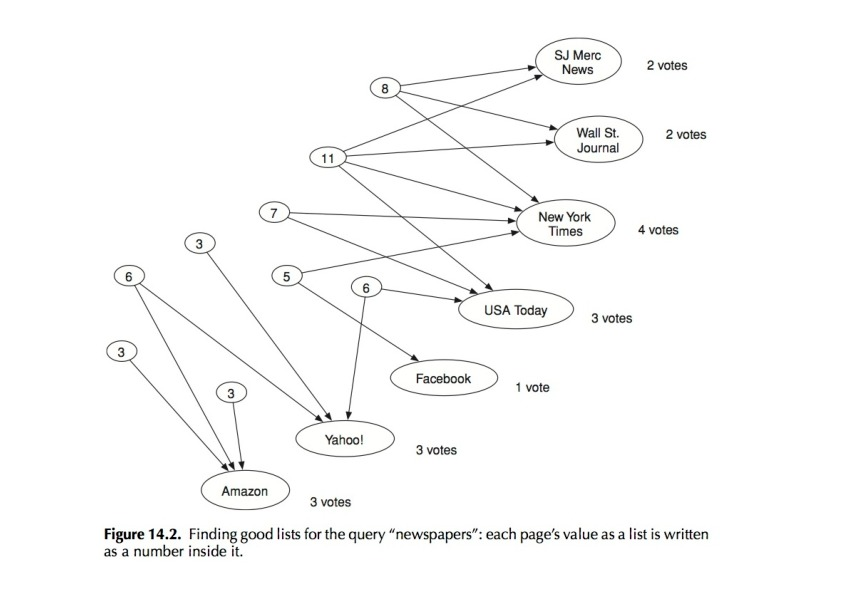
\includegraphics[scale=0.45]{images/ref/fig-14-2.jpeg}
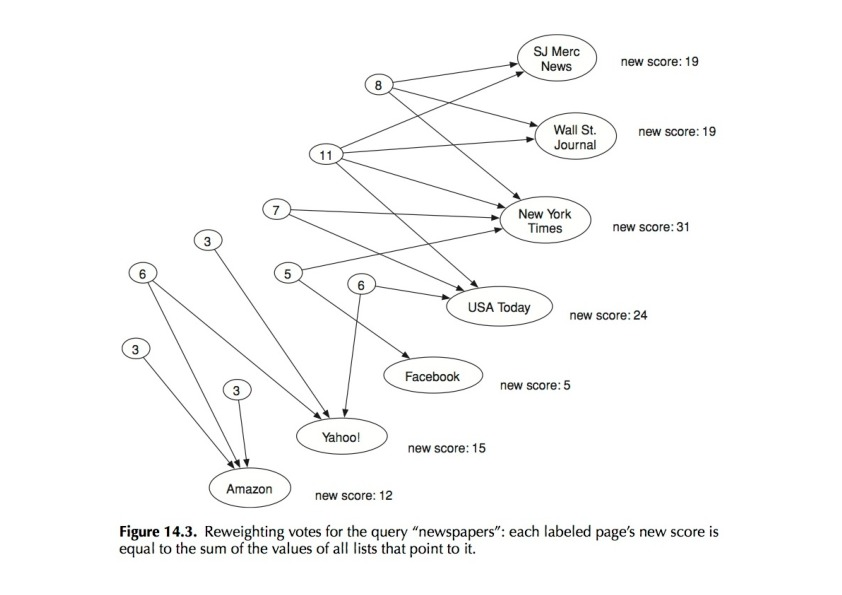
\includegraphics[scale=0.45]{images/ref/fig-14-3.jpeg}
\caption{Page Rank}
\label{pageRankNews1}
\end{figure}

\begin{figure}
\centering

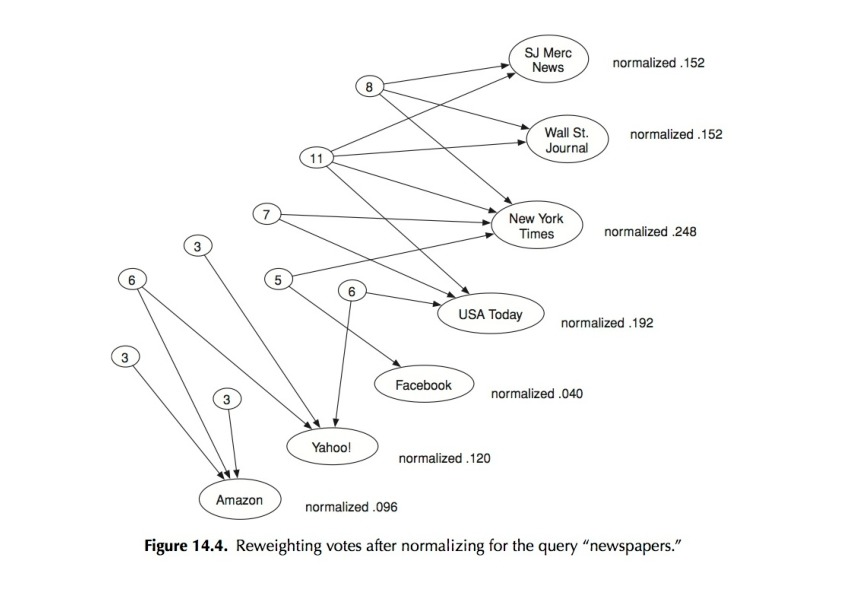
\includegraphics[scale=0.45]{images/ref/fig-14-4.jpeg}
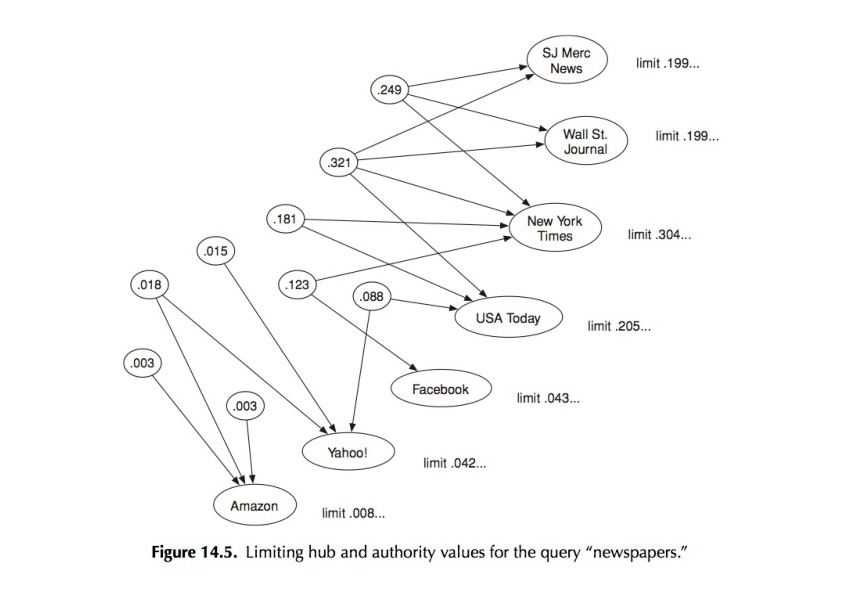
\includegraphics[scale=0.45]{images/ref/fig-14-5.jpeg}
\caption{Page Rank}
\label{pageRankNews2}
\end{figure}



\newpage

	
Comme nous pouvons voir, l'algorithme compte le nombre de liens entrants pour attribuer un poids à chaque place. Puis on normalise les valeurs trouvées, ce qui correspond au poids de la page.
Au plus grand est le poids d'une page au plus son autorité sera grande.

\section{PageRank}
\begin{itemize}
	\item Consolider autorités et concentrateurs.
	\item Une valeur par nœud : son "PageRank" que nous allons calculer. 
	\item Intuition: Un "fluide" qui circule dans le réseau. 
\end{itemize}

\textbf{ Algorithme PageRank :}
\begin{enumerate}
	\item N noeuds (chaque noeud représentant une page) :
	Initialisation Pr(p) =  $\frac{1}{n}$
	\item Choisir un nombre de pas k
	\item K mises à jour:\\
	Pr(p) = $ \sum_ {p'}\frac{Pr(p')}{n(p')} $ avec n(p') le nombre de liens sortant de p' et Pr(p') le poids (ou PageRank) de p' à la $k^{ème}$ itération.
\end{enumerate}
\subsection*{Exemple de PageRank :}

\begin{figure}[h!]
\centering
 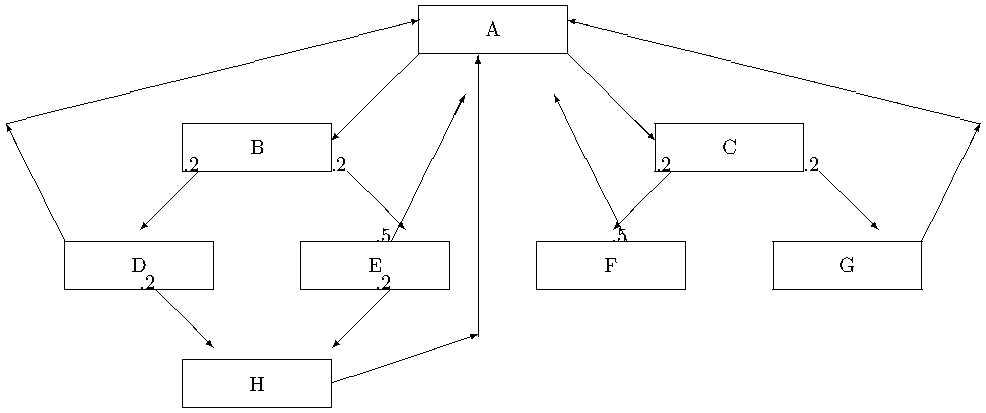
\includegraphics[scale=0.8]{images/24_imagePr.pdf}
\label{graphPageRank}
\end{figure}

 
 	\begin{tabular}{|c| c |c |c |}
		\hline
		Noeuds/Itérations & 0 & 1 & 2 \\
		\hline
		A & 1/8 & 1/2 & 5/16 \\
		B & 1/8 & 1/16 &  1/4   \\
		C & 1/8 & 1/16 & 1/4    \\
		D & 1/8 & 1/16 & 1/32  \\
		E & 1/8 & 1/16 &  1/32   \\
		F & 1/8 & 1/16 & 1/32    \\
		G & 1/8 & 1/16 & 1/32    \\
		H & 1/8 & 1/8 &  1/16   \\
		\hline
		$\sum $ & 1 & 1 & 1 \\
		\hline
	\end{tabular}


 Si nous continuons à laisser travailler l'algorithme, pour un nombre n fini d'itérations telles que k=n, il y aura convergence de l'algorithme. Dans cet exemple-ci,  nous aurons :

	$$Pr(A) = 4/13 ; Pr(B) = 2/13 ; Pr(C) = 2/13 ; Pr(Autres) = 1/13$$
 
Et la condition $\sum Pr(p) = 1$ est toujours vérifiée.
 
 L'équilibre est vérifié si le graphe est connexe,par contre si il ne l'est pas un problème se pose: Le fluide peut arriver au mauvais noeud (analogie réseau d'eau )  :

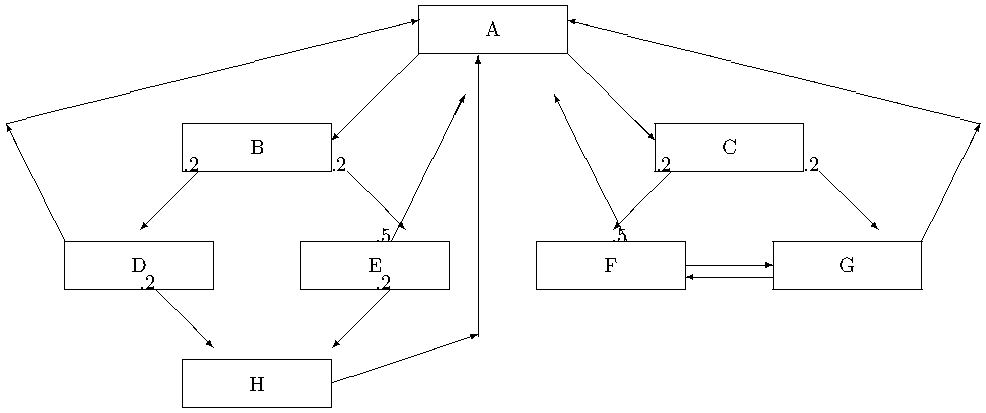
\includegraphics[scale=0.8]{images/24_Nconnexe.pdf}

\subsection*{Solution du problème}
\begin{itemize}
\item Fermer la boucle
\item Créer des cycles
\item Analogie : Circulation d'eau dans l'atmosphère
\end{itemize}
 	La solution est de réinjecter un peu de fluide partout à chaque itération pour éviter que le fluide se concentre dans les noeuds qui n'ont que des liens entrants et pas de liens sortant.

	Ancienne règle de mise à jour :
	\begin{align*}
	Pr(p) =  \sum_ {p'}\frac{Pr(p')}{n(p')}
	\end{align*}
 	Nouvelle règle de mise à jour : \\
	\begin{align*}
         Pr(p) = Sx(Pr(p) + (1-S)  \times \frac{1}{n}) \\
	 \text{Ou S est un paramètre : $ 0 \le S \le 1 $} 
	\end{align*}
        
\subsection*{ Une autre manière de voir l'algorithme:}
        Marche aléatoire d'un utilisateur sur le web : 
	\begin{itemize}
        \item Probabilité de S : Suivre un lien dans la page web ou l'on se trouve \\
        \item (1-S) : Choisi un n\oe ud au hasard, par exemple, taper une adresse URL et accéder directement à un site \\
        \item $\rightarrow $ La même valeur pour Pr(p) \\
	\end{itemize}
	
\subsection*{Historique de PageRank}

	PageRank a commencé à être utilisée au début des années 1990, mais a été en partie abandonné à partir de 2003-2004 pour bloquer les services de SEO (\textit{Search Engine Optimisation}) et autres manipulations du système comme les Google bombs\footnote{wikipedia.org/wiki/Google\_bomb}.
	
	Ceux-ci consistent à altérer les résultats de recherche soit en créant de nombreuses pages contenant des liens vers une page en particulier, soit en utilisant de gros concentrateurs qui contiennent énormément de mots-clés.
	
	Outre les modifications à l'algorithme de tri, certains sites utilisent aussi un attribut html "\textit{nofollow}" qui a pour effet que ces liens n'entrent pas en compte dans le PageRank d'une page. C'est notamment utilisé par les sites de blogging et les sites collaboratifs comme les wikis afin que personne n'ait intérêt à saboter une page pour ajouter un lien et améliorer le classement d'un site en particulier.\footnote{wikipedia.org/wiki/Nofollow}

